\documentclass[stage2a]{tnreport}


\usepackage{dsfont}
\usepackage{glossaries}
\usepackage{enumitem}

\def\reportTitle{Analyse exploratoire des données spatialisées en utilisant des processus ponctuels} % Titre du mémoire
\def\reportLongTitle{Analyse exploratoire des données spatialisées en utilisant des processus ponctuels} % Titre plus long du mémoire

\def\reportAuthor{Clément Dugué}
\def\reportAuthorEmail{\email{clement.dugue@telecomnancy.net}}

\def\reportAuthorAddress{46 rue de Laxou}
\def\reportAuthorCity{54000, NANCY}
\def\reportAuthorPhone{06 11 68 21 32} 

\def\reportIndustrialSupervisor{Radu STOICA}
\def\reportAcademicSupervisor{Sébastien DA SILVA}

\def\reportCompany{Institut Elie Cartan de Lorraine}
\def\reportCompanyAddress{Campus Sciences BP 70239}
\def\reportCompanyCity{54506, VANDOEUVRE LES NANCY}
\def\reportCompanyPhone{03 72 74 54 19}
\def\reportCompanyLogoPath{figures/iecl.png} 

\def\place{Nancy}
\def\date{\today}


\makeglossaries
\newglossaryentry{PP}
{
    name=processus ponctuel,
    description={Type particulier de processus stochastique pour lequel une réalisation est un ensemble de points isolés du temps et/ou de l'espace. Par exemple, la position des arbres dans une forêt peut être modélisée comme la réalisation d'un processus ponctuel}
}

\newglossaryentry{PPoiss}
{
    name=processus de Poisson,
    description={Nommé d'après le mathématicien français Siméon Denis Poisson et la loi du même nom, est un processus de comptage classique dont l'équivalent discret est la somme d'un processus de Bernoulli. C'est le plus simple et le plus utilisé des processus modélisant une file d'attente. C'est un processus de Markov, et même le plus simple des processus de naissance et de mort}
}

\newglossaryentry{PPPoiss}
{
    name=processus ponctuel de Poisson,
    description={Le processus ponctuel de Poisson est le plus simple et le plus universel des \gls{PP}*. C'est une généralisation spatiale du \gls{PPoiss}* utilisé en théorie des files d'attentes}
}

\newglossaryentry{stationnaire}
{
    name=stationnaire,
    description={Dont les propriétés ne changent pas selon l'endroit où l'on regarde}
}

\newglossaryentry{homogene}
{
    name=homogène,
    description={Dont les propriétés ne changent pas au cours du temps}
}

\newglossaryentry{realisation}
{
    name=réalisation,
    description={La réalisation d'un processus ponctuel est un ensemble de points isolés du temps et/ou de l'espace. Par exemple, la position des arbres dans une forêt peut être modélisée comme la réalisation d'un processus ponctuel}
}

\newglossaryentry{statDescriptive}
{
    name=statistique descriptive,
    description={Technique utilisée pour décrire un ensemble relativement important de données}
}

\newglossaryentry{spatstat}
{
    name=librairie spatstat,
    description={Librairie fournissant des méthode de calcul pour l'étude de statistiques spatiales, spatstat est plutôt orienté vers les calculs en 2 Dimensions}
}

\newglossaryentry{double}
{
    name=double,
    description={Nombre codés sur 64 bits entre \begin{math}-1.7*10^{-308} \end{math} et \begin{math}1.7*10^{308}\end{math} }
}

\newglossaryentry{namespace}
{
    name=namespace,
    description={Lieu abstrait conçu pour accueillir des ensembles de termes appartenant à un même répertoire}
}

\newglossaryentry{classe}
{
    name=classe,
    description={En programmation orientée objet, la déclaration d'une classe regroupe des membres, \gls{classe}s* et attributs (variables) communs à un ensemble d'objets. Il est possible de restreindre l'ensemble d'objets représenté par une classe A grâce à un mécanisme d'\gls{heritage}age*. Dans ce cas, on crée une nouvelle classe B liée à la classe A et qui ajoute de nouvelles propriétés}
}

\newglossaryentry{instance}
{
    name=instance,
    description={En programmation orientée objet, on appelle instance d'une \gls{classe}*, un \gls{objet}* avec un comportement et un état, tous deux définis par la \gls{classe}*. Il s'agit donc d'un \gls{objet}* constituant un exemplaire de la \gls{classe}*}
}

\newglossaryentry{objet}
{
    name=objet,
    description={En programmation orientée objet, un objet est créé à partir d'une \gls{classe}*, de laquelle il \gls{heritage}e* les comportements et les caractéristiques}
}

\newglossaryentry{methode}
{
    name=méthode,
    description={En programmation orientée objet, une méthode est une entité informatique dans une \gls{classe}* qui encapsule une portion de code effectuant un traitement spécifique bien identifié (asservissement, tâche, calcul, etc.)}
}

\newglossaryentry{heritage}
{
    name=héritage,
    description={En programmation orientée objet, l’héritage est un mécanisme qui permet, lors de la déclaration d’une nouvelle \gls{classe}*, d'y inclure les caractéristiques d’une autre \gls{classe}*}
}

\newglossaryentry{richardson}
{
    name=extrapolation de Richardson,
    description={En analyse numérique, le procédé d'extrapolation de Richardson est une technique d'accélération de la convergence. Il est ainsi dénommé en l'honneur de Lewis Fry Richardson, qui l'a introduit au début du XXe siècle}
}

\newglossaryentry{trapeze}
{
    name=méthode des trapèzes,
    description={Méthode pour le calcul numérique d'une intégrale, qui calcule l'aire des trapèzes successifs sous la courbe d'une fonction}
}



\begin{document}
  
\maketitle
\pagenumbering{roman}

\insertAntiPlagiarismAgreement{Dugué, Clément}{2406037702x}

\cleardoublepage

\makesecondtitle

\section*{Remerciements}
\addcontentsline{toc}{chapter}{Remerciements}

{\em
En premier lieu, je tiens à remercier M. Xavier ANTOINE directeur de l'institut Elie Cartan et M. Antoine Lejay responsable de l'équipe de Probabilités Statistiques pour m'avoir accueilli dans le laboratoire.\\

J'adresse également mes remerciements à mon maître de stage M. Radu STOICA pour ses explications, son soutien et son écoute tout au long du stage, ainsi que pour la confiance qu'il m'a accordée en m'acceptant comme stagiaire.\\

Je souhaite aussi remercier mon encadrant universitaire M. Sébastien DA SILVA qui a participé au bon déroulement de ce stage.\\

Je remercie enfin toutes les personnes m'ayant aidé dans l'écriture et la relecture de ce rapport de stage.
}

\cleardoublepage

\renewcommand{\baselinestretch}{0.5}\normalsize
\tableofcontents
\renewcommand{\baselinestretch}{1.0}\normalsize
\cleardoublepage

\pagenumbering{arabic}
\setcounter{page}{1}

\chapter{Introduction}


Lors de l'étude d'un phénomène (localisation d'évènements historiques, de micro-organismes, de populations...), les données spatialisées synthétisent l'information relative à la position. On peut représenter ces données sous forme de points. On obtient ainsi une représentation des données sur laquelle il est plus facile de raisonner. Par l'analyse statistique, on peut alors identifier des tendances selon la densité des points (si les points sont rapprochés ou non). Les résultats de l'analyse peuvent ensuite être interprétés pour en tirer des conclusions, et fournir ainsi des informations objectives utiles pour de nombreux domaines.

L'automatisation de cette analyse se fait par la création de programmes informatiques qui peuvent lire les données fournies et faire des calculs rapides.
Cependant il n'y a pas de solution toute faite pour l'analyse statistique de répartition de points, en effet chaque cas doit être analysé en fonction de son contexte (obtention des données, objectif de l'analyse). D'où le besoin de fonctions et de programmes multiples pour cette analyse.

Ce fut le but de ce stage: créer des outils informatiques pour traiter et analyser des données ponctuelles selon des méthodes mathématiques fournies et expliquées par mon tuteur.
La réalisation des fonctions se faisait en plusieurs étapes: d'abord la lecture et compréhension de la documentation sur la fonction, puis la conception et l'écriture du code, et enfin une analyse des résultats obtenus en vue d'une amélioration (retour à la 2ème étape). Ainsi, après une présentation globale de l'entreprise d'accueil, la structure de ce rapport suivra l'enchaînement des étapes présentées ci-dessus. 

Enfin les termes spécifiques et définitions, seront réunies dans le glossaire (page 30). Dans le texte, un * renvoie à ce glossaire.

\newpage

\chapter{Présentation de l'entreprise d'accueil}

\section{Institut Elie Cartan}

La recherche lorraine en mathématiques est présente en lorraine depuis l'arrivée d'Élie Cartan il y a une centaine d'année. Elle a été marquée par une succession de personnalités de renommée mondiale comme Jean Leray, Laurent Schwartz (Médaille Fields 1950), Jean-Pierre Serre (Médaille Fields 1954), Roger Godement, Jean Delsarte (secrétaire du groupe Bourbaki jusqu’en 1962) ou Jacques-Louis Lions.

Créé en 1953 à l’initiative de Jean Delsarte, l’Institut Élie Cartan de Nancy a été reconnu par le CNRS en 1978 (sous le nom d’Équipe d’Analyse Globale) et il a fusionné avec le Laboratoire de Mathématiques et Applications de Metz au premier janvier 2013. Le nouveau laboratoire est intitulé Institut Elie Cartan de Lorraine (IECL),

\section{L'IECL}

D'après son site internet~\cite{Presentation}, l’IECL est une unité mixte de recherche (UMR 7502) du CNRS et de l’Université de Lorraine. L’INRIA est un partenaire important et de longue date de l’IECL, notamment à travers les équipes-projets INRIA que nous hébergeons.

Avec environ 120 enseignants-chercheurs et chercheurs permanents, l’Institut Élie Cartan de Lorraine est l’un des grands laboratoires français en mathématiques et le plus grand de l’Est de la France.

 Dans plusieurs domaines des mathématiques fondamentales (géométrie, théorie des nombres), des équations aux dérivées partielles ou des probabilités, l’IECL rassemble des spécialistes reconnus internationalement. Cette diversité scientifique favorise les interactions internes et externes, en contribuant à l’attractivité pour les visiteurs étrangers.

\newpage

\section{L'équipe Probabilités et Statistiques}

L’équipe de Probabilités et Statistique est l’une des quatre équipes de l’IECL. Forte d’une trentaine de membres, elle accueille en son sein les équipes projet INRIA Bigs et Tosca.

Son effectif relativement important (une trentaine de permanents) en fait une des plus grosses équipes du territoire français. Cela lui permet de couvrir l’essentiel du spectre de la recherche contemporaine en probabilités et statistique, comme par exemple l’étude de structures probabilistes discrètes (graphes, arbres), la modélisation et estimation avec des applications par exemple à la biologie, la médecine, la finance, le comportement en temps long des processus stochastiques, les trajectoires rugueuses, la simulation Monte Carlo.

De nombreux membres sont impliqués dans des collaborations inter-disciplinaires en France ou à l’étranger, et/ou industrielles.


\newpage

%%%%%%%%%%%%%%%%%%%%%%%%%%%%%%%%%%%%%%%%%%%%%%%%%%%%%%%%%%%%%

\chapter{Problématique : présentation du problème }


\section{Contexte} 

Étant membre de l'équipe Proba-Stats, mon maître de stage M. Radu Stoica étudie les \gls{PP}s* (répartitions de points). Ayant réalisé en langage C et C++ des fonctions simulant des répartitions de points, il souhaitait alors pouvoir analyser ces processus.\\

Des librairies d'analyse existent sous R comme la \gls{spatstat}*, mais sont limitées: ces méthodes ne sont pas applicables pour des jeux de données plus larges. Ainsi mon maître de stage souhaitait avoir ces librairies d'analyse en C et C++ afin de pouvoir gérer des données plus complexes. De plus cette implémentation permet d'envisager une extension en trois dimensions qui n'est pas encore mise en place dans la \gls{spatstat}*. Il sera alors possible d'étudier des modèles plus réalistes.

J'ai eu à lire et interpréter la partie théorique au fur et à mesure des créations des fonctions. Dans un soucis de clarté, je vais commencer par expliquer l'intensité d'un \gls{PP}*. 

%%%%%%%%%%%%%%%%%%%%%%%%%%

\section{Intensité d'un processus ponctuel}

Pour un \gls{PP}*, l'intensité donne une mesure du nombre moyen de points sur une surface.

Soit X un \gls{PP}* sur \begin{math} \mathbb{R}^2\end{math} et soit \textbf{x} une \gls{realisation}* de X observé dans \begin{math} W \subseteq \mathbb{R}^2\end{math}. Pour chaque sous-région B de W, on s'intéresse à la formule:
\begin{align*}
    \mathbb{E}[n(\textbf{x} \cap B)] = \int_B \lambda(u) \, \mathrm du
\end{align*}

Ainsi si l'intensité est \gls{homogene}* sur W, le nombre de points de \textbf{x} dans B est censé être proportionnel à l'aire de B:
\begin{align*}
    \mathbb{E}[n(\textbf{x} \cap B)] = \lambda |B|
\end{align*}
où \begin{math}\lambda\end{math} est une constante qu'on appelle "intensité".

L'intensité \begin{math}\lambda\end{math} est le nombre de points prévus dans chaque sous-région B. Si X est \gls{homogene}* on peut alors estimer \begin{math}\lambda\end{math} telle que:
\begin{align*}
    \hat{\lambda} = \frac{n}{|W|}
\end{align*}
avec n le nombre de points présents dans W.

Cependant si l'intensité n'est pas \gls{homogene}*, il faut l'estimer différemment. Une méthode est l'estimation par noyau. Le principe est de quadriller la surface W et pour chaque maille u du quadrillage de chercher l'influence qu'elle amène en étudiant la densité de point dans son voisinage avec une fonction de noyau k:
\begin{align*}
    \hat{\lambda}(u) = \sum_{i=1}^n k(u-x_i)
\end{align*}

La fonction de noyau k est une densité de probabilité, ainsi pour toute maille u du quadrillage la fonction doit respecter les propriétés:
\begin{center}
\begin{minipage}{5cm}
%\begin{itemize}[label=$\square$]
\begin{itemize}[label=\textbullet]
    \item \begin{math} k(u) \geq 0 \end{math}
    \item \begin{math} \int_{\mathbb{R}^2} k(u) \, \mathrm du = 1\end{math}
\end{itemize}
\end{minipage}
\end{center}
Il y a alors plusieurs manières de définir la fonction noyau, on s'intéressera pour l'implémentation aux fonctions suivantes.

\begin{minipage}{0.6\linewidth}
Noyau carré:\begin{math}\quad k(u_1,u_2) = \displaystyle\frac{1}{c^2} \  \mathds{1}\{ |u_1| < c/2 \  , \, |u_2| < c/2  \} \end{math}

\vspace{1.5cm}

Noyau disque:\begin{math}\quad k(u_1,u_2) = \displaystyle\frac{1}{\pi r^2} \  \mathds{1} \left \{ \sqrt{u_1^2 + u_2^2} \leq r \right \} \end{math}

\vspace{1.5cm}

Noyau gaussien:\begin{math}\quad k(u_1,u_2) = \displaystyle\frac{1}{2 \pi \sigma} \  exp \left [ -\displaystyle\frac{u_1^2 + u_2^2}{2 \sigma^2} \right ] \end{math}\\
(image prise sur le site \cite{Gauss})

\end{minipage}\hfill
\begin{minipage}{0.35\linewidth}
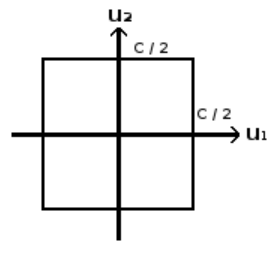
\includegraphics[scale=0.3]{figures/carre.png}\\
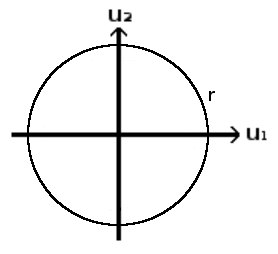
\includegraphics[scale=0.3]{figures/rond.png}
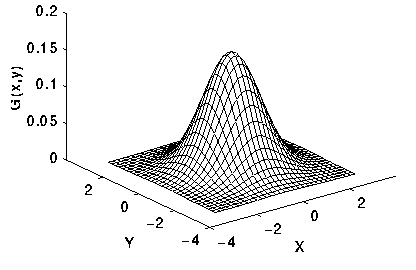
\includegraphics[scale=0.3]{figures/gaussien.png}
\end{minipage}


Enfin, des défauts d'estimation vont apparaitre lorsque l'on s'approche des bords de W : les effets de bord. En effet les points de \textbf{x} en dehors de la surface W étudiée ne seront pas pris en compte. Afin de remédier à ce problème, on peut appliquer la correction de Diggle. En notant, pour chaque point de la surface W, la correction à appliquer:
\begin{align*}
e(x_i) = \int_W K(u-v) \, \mathrm dv 
\end{align*} 
La correction de Diggle consiste à compenser les effets de bords pour chaque point tel que: 
\begin{align*}
    \hat{\lambda}(u) = \sum_{i=1}^n \frac{1}{e(x_i)} k(u-x_i)
\end{align*}

%%%%%%%%%%%%%%%%%%%%%%%%%%
\section{L'analyse de processus ponctuels}

Dans le cadre de l'analyse des \gls{PP}s*, on identifie de manière générale trois grandes tendances représentées dans la figure~\ref{fig:repartition}:
\begin{itemize}
\item répulsive (les points se trouvent à une certaine distance les uns des autres);
\item aléatoire (les points n'ont pas de dépendance);
\item agrégée (les points forment des groupes de points).
\end{itemize}

\begin{figure}[h]
  \centering
  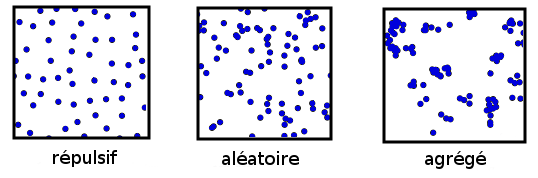
\includegraphics[scale=0.6]{figures/repartition2.png}
  \caption{Représentation des différentes formes de représentations spatiales de points}
  \label{fig:repartition}
\end{figure}

Une manière statistique de déterminer si une observation de points correspond à l'un ou l'autre de ces trois cas, est de mesurer son écart avec un \gls{PPPoiss}*. En effet ce type de \gls{PP}* à la propriété de répartir ses points d'une manière totalement aléatoire.

%%%%%%%%%%%%

\section{La fonction K}

\subsection{Principe}
Supposons qu'on se pose une question sur l'espacement entre les points dans un ensemble de points. Il serait alors naturel de regarder les distances entre chaque point. Si ces distances sont plutôt grandes, la répartition des points sera plutôt répulsive. Alors que si elles sont plutôt petites, la répartition des points sera plutôt agrégée.

\subsection{La fonction K empirique}

Soit X un \gls{PP}* \gls{stationnaire}* sur \begin{math} \mathbb{R}^2\end{math} d'intensité \begin{math}\lambda\end{math} et soit \textbf{x} une \gls{realisation}* de X observée dans \begin{math} W \subseteq \mathbb{R}^2\end{math}. Les distances \begin{math} d_{ij} = ||x_i-x_j||\end{math} entre chaque point distinct \begin{math} x_i \end{math} et \begin{math} x_j \end{math} de \textbf{x} constituent une \gls{statDescriptive}*.
La fonction K empirique est définie pour chaque distance \begin{math} r \geq 0 \end{math} par la formule:
\begin{align*}
\hat{K}(r) = \frac{1}{n \lambda} \sum_{i=1}^n \sum_{\underset{j \neq i}{j=1}}^n \mathds{1} \{d_{ij} \leq r \}
\end{align*}
La fonction indicatrice  \begin{math} \mathds{1} \{...\}\end{math} vaut 1 si son contenu est vrai et 0 sinon. La somme de ces indicatrices est simplement le nombre de fois où le contenu est vrai.\\

\begin{wrapfigure}{r}{7.5cm}
\vspace{-1.2cm}
\begin{center}
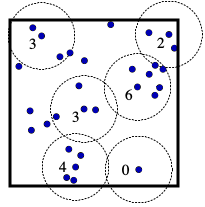
\includegraphics[width=5.5cm]{figures/nombreVoisins2.png}
\caption{Nombre de points voisins dans un certain rayon.}
\label{fig:nombreVoisins}
\end{center}
\end{wrapfigure}

La fonction K est une moyenne normalisée du nombre de voisins dans une boule de rayon r, sans compter le point lui même. Ces nombres de points voisins sont représentés sur la figure~\ref{fig:nombreVoisins}. La normalisation est représentée dans la formule par le facteur \begin{math}1/\lambda\end{math}. Comme vu dans son paragraphe dédié,  l'intensité du processus \begin{math}\lambda\end{math} est une mesure du nombre moyen de point dans W. On peut ici l'estimer par |W|/(n-1).\\

%%%%%%%%%%%%

\subsection{La fonction K pour un processus de Poisson stationnaire}

\begin{wrapfigure}[11]{r}{7.5cm}
\vspace{-1.4cm}
\begin{center}
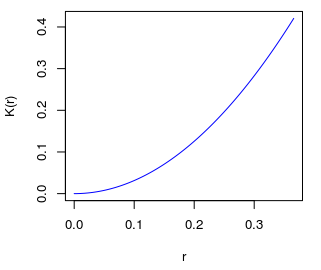
\includegraphics[width=6.5cm]{figures/Kpoiss2.png}
\caption{Représentation de la fonction K pour une répartition totalement aléatoire.}
\label{fig:Kpoiss}
\end{center}
\end{wrapfigure} 

En suivant la partie 7.3.2 du livre \textit{Spatial Point Patterns - Methodology and Applications with R}~\cite{BaddEtal16}, on peut montrer que la fonction estimée par \begin{math}\hat{K}(r)\end{math} est donnée par:
\begin{align*} K_{pois}(r) = \pi r^2 \end{align*}
pour un \gls{PPoiss}* \gls{stationnaire}*.

La figure~\ref{fig:nombreVoisins} montre alors la représentation en fonction de r de la fonction K théorique.

%%%%%%%%%%%%

\vspace{0.5cm}
\subsection{Interprétation de K}
La figure~\ref{fig:interpretK} ci dessous montre la fonction estimée de K pour les 3 configurations de la section 3.3 (figure~\ref{fig:repartition}) selon que la configuration est agrégée, aléatoire ou bien répulsive. Les courbes rouges représentent \begin{math}\hat{K}\end{math} tandis que les courbes bleues discontinues représentent \begin{math}K_{pois}\end{math}.\\

\begin{figure}[h]
  \centering
  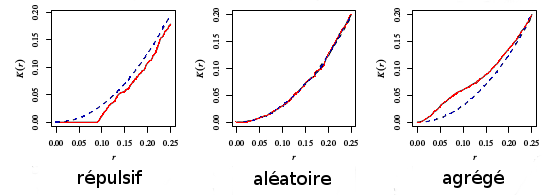
\includegraphics[scale=0.7]{figures/interpretK2.png}
  \caption{Différentes estimations de K.}
  \label{fig:interpretK}
\end{figure}


Sur la gauche, la courbe de la fonction calculée est en dessous de celle pour une répartition totalement aléatoire (\begin{math}\hat{K}(r) < K_{pois}(r) \end{math}). Ainsi, pour une distance r, un point quelconque a en moyenne moins de voisins qu'il aurait pu espérer avoir avec une répartition totalement aléatoire. Donc la répartition semble plutôt répulsive.\\
\indent
Sur la droite, la courbe de la fonction calculée est au dessus de celle pour une répartition totalement aléatoire (\begin{math}\hat{K}(r) > K_{pois}(r) \end{math}). Ainsi, pour une distance r, un point quelconque a en moyenne plus de voisins qu'il aurait pu espérer avoir avec une répartition totalement aléatoire. Donc la répartition semble plutôt agrégée.\\


%%%%%%%%%%%%%%%%%%%%%%%%%%%%%%%%%%%%%%%%%%%%%%%%%%%%%%%%%%%%%%%%
%%%%%%%%%%%%%%%%%%%%%%%%%%%%%%%%%%%%%%%%%%%%%%%%%%%%%%%%%%%%%%%%


\section{Fonction d'espace vide F}

\subsection{Définitions pour un processus de point stationnaire}

Soit X un \gls{PP}* sur \begin{math}\mathbb{R}^2\end{math} d'intensité \begin{math}\lambda\end{math} et soit \textbf{x} une \gls{realisation}* de X observée dans \begin{math} W \subseteq \mathbb{R}^2\end{math}. On note d(u,\textbf{x}) la distance d'une position \begin{math} u \in \mathbb{R}^2 \end{math} au plus proche point de \textbf{x}. Cette fonction est appelé 'distance d'espace vide' et est définie par:
\begin{center}\begin{math} d(u,\textbf{x}) = min\{ ||u-x_i|| : x_i \in \textbf{x} \} \end{math}\end{center}

La fonction F de distance d'espace vide est définie pour toute distance \begin{math} r \geq 0 \end{math} par:
\begin{center}\begin{math} F(r) = \mathbb{P}\{ d(u,\textbf{x}) \leq r \} \end{math}\end{center}

Les valeurs de F(r) sont des probabilités, elles sont comprises entre 0 et 1. Elles définissent les chances de trouver un point dans un disque de rayon r sur la surface étudiée.\\

%%%%%%%%%%%%%%%%

\subsection{La fonction F pour un processus de Poisson stationnaire}

\begin{wrapfigure}[9]{r}{7.5cm}
\vspace{-0.8cm}
\begin{center}
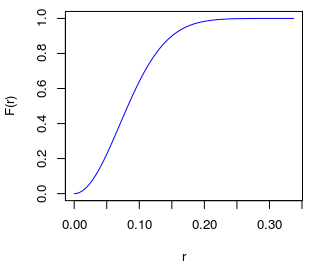
\includegraphics[width=6cm]{figures/poisson2.png}
\caption{Représentation de la fonction de répartition de Poisson pour $\lambda$ = 40.}
\label{fig:poisson}
\end{center}
\end{wrapfigure}

Pour un \gls{PPoiss}* \gls{stationnaire}* d'intensité \begin{math}\lambda\end{math}, on peut calculer:
\begin{align*}
F_{pois}(r) &= \mathbb{P}\{d(u,\textbf{x}) \leq r\} \\
            &= \mathbb{P}\{n( b(u,r) \cap \textbf{x} ) \neq 0\} \\
            &= 1 - \mathbb{P}\{ n( b(u,r) \cap \textbf{x} ) = 0\} \\
            &= 1 - exp(-\lambda \pi r^2)
\end{align*}
car par stationnarité, F(r) ne dépend pas de u. La figure~\ref{fig:poisson} montre la représentation en fonction de r de cette fonction théorique.\\


%%%%%%%%%%%%%%%%

\subsection{Estimation de F}

Pour estimer la fonction F à partir de la \gls{realisation}* \textbf{x} finie, on doit discrétiser pour obtenir les valeurs de u considérées. Ainsi pour n'importe quelle position \textit{u} sur la surface W à analyser, on mesure la distance \textit{d(u,}\textbf{x}\textit{)} la séparant du point voisin le plus proche (distance d'espace vide). On répète alors cette opération pour un nombre m de positions \begin{math}u_1\end{math},...,\begin{math}u_m\end{math} équitablement réparties sur la surface. On peut alors calculer la fonction empirique comme fonction sur la distance \begin{math} r \geq 0 \end{math}:
\begin{align*} \hat{F}(r) = \frac{1}{m}\sum_{j=1}^m \mathds{1} \{d(u_j,\textbf{x}) \leq r \}\end{align*}


%%%%%%%%%%%%%%%%

\subsection*{Interprétation de F}

La figure~\ref{fig:interpretF} ci dessous montre la fonction estimé de F pour les 3 configurations de la section 3.3 (figure~\ref{fig:repartition}) selon que la répartition est agrégée, aléatoire ou bien répulsive. Les traits discontinus sont la représentation graphique de la fonction F théorique pour un aléatoire total.

\begin{figure}[h]
  \centering
  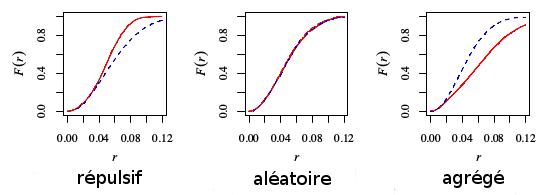
\includegraphics[scale=0.7]{figures/interpretF2.png}
  \caption{Différentes estimations de F.}
  \label{fig:interpretF}
\end{figure}

Sur la gauche, la courbe de la fonction calculée est au dessus de celle pour une répartition totalement aléatoire (\begin{math}\hat{F}(r) > F_{pois}(r) \end{math}). Ainsi, pour une distance r, la probabilité  \begin{math} \mathbb{P}\{d(u,\textbf{x}) \leq r\} \end{math} est plus grande quelle ne l'est pour une répartition aléatoire, les espaces vides sont donc plus petits que prévu. Donc la répartition semble plutôt répulsive.

Sur la droite, la courbe de la fonction calculée est en dessous de celle pour une répartition totalement aléatoire (\begin{math}\hat{F}(r) < F_{pois}(r) \end{math}). Ainsi, pour une distance r, la probabilité que \begin{math} \mathbb{P}\{d(u,\textbf{x}) \leq r\} \end{math} est plus petite quelle ne l'est pour une répartition aléatoire, les espaces vides sont donc plus grands que prévu. Donc la répartition semble plutôt agrégée.


%%%%%%%%%%%%%%%%%%%%%%%%%%%%%%%%%%%%%%%%%%%%%%%%%%%%%%%%%%%%%%%

\section{La fonction G du plus proche voisin}

\subsection{Définitions pour un processus de point stationnaire}

Soit X un \gls{PP}* \gls{stationnaire}* sur \begin{math} \mathbb{R}^2\end{math} d'intensité \begin{math}\lambda\end{math} et soit \textbf{x} une \gls{realisation}* de X observée dans \begin{math} W \subseteq \mathbb{R}^2\end{math}. La distance du plus proche voisin d'un point \begin{math}x_i\end{math} de \textbf{x} est écrite telle que:
\begin{center}\begin{math} d_i = d(x_i,\textbf{x}\backslash x_i ) \end{math}\end{center}
C'est la plus courte distance de \begin{math} x_i \end{math} à un autre point de \textbf{x} excepté \begin{math} x_i \end{math}.

La fonction G de distance du plus proche voisin est alors définie pour toute distance \begin{math} r \geq 0 \end{math} telle que:
\begin{center}\begin{math} G(r) = \mathbb{P}\{ d(u,\textbf{x}\backslash u) \leq r | \text{ u est un point de \textbf{x}} \} \end{math}\end{center}

%%%%%%%%%%%%%%%%

\subsection{Valeurs pour un aléatoire complet}
Pour un \gls{PPoiss}* \gls{stationnaire}* \gls{homogene}* d'intensité \begin{math}\lambda\end{math}, il est possible de prouver que la fonction G est égale à la fonction d'espace vide F: 
\begin{center}\begin{math} F_{pois}(r) = G_{pois}(r) = 1 - exp(-\lambda \pi r^2) \end{math}\end{center}
Cela n'est vrai que pour une répartition totalement aléatoire, en général F et G seront des fonctions différentes.

%%%%%%%%%%%%%%%%

\subsection{Estimation de G}

Pour un point \begin{math}x_i\end{math} de \textbf{x}, on mesure la distance \begin{math}d_i = d(x_i,\textbf{x}\end{math}\textbackslash\begin{math} x_i)\end{math} la séparant du point voisin le plus proche (distance du plus proche voisin). On répète alors cette opération pour tous les points \begin{math}x_1\end{math},...,\begin{math}x_n\end{math} de la configuration, avec n le nombre des points. On peut alors calculer la fonction empirique pour toute distance \begin{math} r \geq 0 \end{math} telle que:
\begin{align*} \hat{G}(r) = \frac{1}{n}\sum_{i=1}^n \mathds{1} \{d_i \leq r \}\end{align*}

%%%%%%%%%%%%%%%%

\subsection{Interprétation de G }

La figure~\ref{fig:interpretG} ci-dessous montre la fonction estimée de G pour les 3 configurations de la section 3.3 (figure~\ref{fig:repartition}) selon que la répartition est agrégée, aléatoire ou bien répulsive. Les traits discontinus sont la représentation graphique de la fonction G théorique pour un aléatoire total.

\begin{figure}[h]
  \centering
  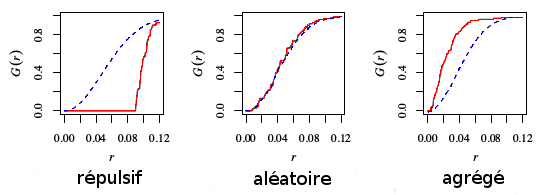
\includegraphics[scale=0.7]{figures/interpretG2.png}
  \caption{Différentes estimations de G.}
  \label{fig:interpretG}
\end{figure}

Sur la gauche, la courbe de la fonction calculée est en dessous de celle pour une répartition totalement aléatoire (\begin{math}\hat{G}(r) < G_{pois}(r) \end{math}). Ainsi, pour une distance r, la probabilité  \begin{math} \mathbb{P}\{ d(u,\textbf{x}\backslash u) \leq r | \text{ u est un point de \textbf{x}} \} \end{math} est plus petite quelle ne l'est pour une répartition aléatoire, les points ont des voisins plus éloignés que prévus. Donc la répartition semble plutôt répulsive.

Sur la droite, la courbe de la fonction calculée est au dessus de celle pour une répartition totalement aléatoire (\begin{math}\hat{G}(r) > G_{pois}(r) \end{math}). Ainsi, pour une distance r, la probabilité que \begin{math} \mathbb{P}\{ d(u,\textbf{x}\backslash u) \leq r | \text{ u est un point de \textbf{x}} \} \end{math} est plus grande quelle ne l'est pour une répartition aléatoire, les points ont des voisins plus proches que prévus. Donc la répartition semble plutôt agrégée.

%%%%%%%%%%%%%%%%

\section{Fonction J}

Les distances du plus proche voisin et les distances d'espace-vide ont la même distribution de probabilité si la répartition des points est totalement aléatoire (pour un processus de Poisson*). Les fonctions F et G ont tendance à s'écarter de la fonction de Poisson de façon opposée: l'une devient plus grande et l'autre plus petite. Cela suggère qu'une combinaison de ces 2 types de distances pourrait être utile pour évaluer une répartition.\\
Une combinaison pratique de G et F, suggérée par la théorie fondamentale, est la fonction J d'un \gls{PP}* \gls{stationnaire}*:
\begin{center}\begin{math} J(r) = \frac{1-G(r)}{1-F(r)} \end{math}\end{center}
définie pour tout \begin{math} r \geq 0 \end{math} telle que F(r) < 1. Pour un \gls{PPoiss}* \gls{homogene}*, \begin{math} F_{pois} \equiv G_{pois} \end{math} ainsi les valeurs de J(r) > 1 sont cohérentes avec une représentation répulsive, tandis que les valeurs de J(r) < 1 sont cohérentes avec une représentation agrégée.


%%%%%%%%%%%%%%%%

\section{Effet des bords}

\subsection{Principe}
Les calculs de F, G et K donnés précédemment ne sont pas tout à fait exacts. En effet, ne prenant pas en compte les points qui seraient en dehors d'une \gls{realisation}*, les calculs sur les bords de la surface seront erronés.\\
Une stratégie simple pour corriger ces problèmes d'estimation est la méthode de restriction des bords. Par exemple, lorsqu'on fait une estimation de K(r) pour une distance r, on limite les calculs aux points se trouvant à une distance r du bord de la surface étudiée. Ainsi le cercle de rayon r autour du point loge entièrement dans la surface comme le montre la figure~\ref{fig:bords}.

\begin{figure}[h]
  \centering
  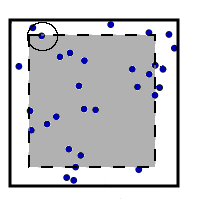
\includegraphics[scale=0.5]{figures/bords2.png}
  \caption{Exemple de zone de sûreté pour un certain rayon.}
  \label{fig:bords}
\end{figure}

%%%%%%%%%%%%%%%%

\subsection{Correction pour K}

En prenant en compte que les points sont dans la zone de sûreté pour chaque r, on peut alors réécrire \begin{math} \hat{K}(r) \end{math}. En gardant les mêmes notations qu'au 3.3.2 (La fonction K empirique), on peut écrire la fonction K avec correction des bords \begin{math} \hat{K}_{bord}(r) \end{math} telle que:
\begin{align*}
\hat{K}_{bord}(r) = \frac{  \sum_{i=1}^n \mathds{1} \{b_i \geq r \} \sum_{\underset{j \neq i}{j=1}}^n \mathds{1} \{d_{ij} \leq r \}}{\lambda \sum_{i=1}^n \mathds{1} \{b_i \geq r \}}
\end{align*}
où \begin{math}b_i\end{math} est la distance d'un point \begin{math}x_i\end{math} au bord de la surface.

%%%%%%%%%%%%%%%%

\subsection{Correction pour F}

La même méthode de restriction des bords peut être appliquée à \begin{math} \hat{F}(r) \end{math}. Pour cette fonction, on ne se limite non pas aux points, mais aux positions \textit{u} qui sont à une distance du bord de la surface supérieure à r. Ainsi en gardant les mêmes notations qu'au 3.4.3 (Estimation discrète de F), on peut écrire la fonction F avec correction des bords:
\begin{align*}
\hat{F}_{bord}(r) = \frac{  \sum_{j=1}^m \mathds{1} \{d(u_j,\textbf{x}) \leq r \} \mathds{1} \{b_j > r \} }{ \sum_{j=1}^m \mathds{1} \{b_j > r \}}
\end{align*}
où \begin{math}b_j\end{math} est la distance d'une position \begin{math}u_j\end{math} au bord de la surface.

%%%%%%%%%%%%%%%%

\subsection{Correction pour G}

Pour appliquer la restriction des bords à \begin{math} \hat{G}(r) \end{math}, on se limite comme pour K aux points qui sont à une distance du bord de la surface supérieure à r. Ainsi en gardant les mêmes notations qu'au 3.5.3 (Estimation discrète de G), on peut écrire la fonction G avec correction des bords:
\begin{align*}
\hat{G}_{bord}(r) = \frac{  \sum_{i=1}^n \mathds{1} \{d_i \leq r \} \mathds{1} \{b_i \geq r \} }{ \sum_{i=1}^n \mathds{1} \{b_i \geq r \}}
\end{align*}
où \begin{math}b_i\end{math} est la distance d'un point au bord de la surface.

%%%%%%%%%%%%%%%%

\section{Test d'enveloppe}

Les estimations des fonctions F, G, J et K sont faites à partir de \gls{realisation}s*. Cela induit un écart entre la valeur théorique et la valeur estimée. La question que l'on se pose est: est-ce que la configuration observée pourrait être considérée comme la \gls{realisation}* d'un \gls{PPoiss}*? Pour cela on fait appel au test d'enveloppe: un outil fournissant une meilleure estimation pour répondre à la question. Son principe est le suivant:
on lance les calculs des fonctions F, G, J et K sur un nombre n de configurations de points que l'on sait être aléatoires. On regarde ensuite les valeurs des n courbes obtenues. On peut tracer les courbes représentant les minimums et maximums atteints par les fonctions sur chaque abscisse. On obtient alors une enveloppe de toutes les valeurs obtenues pour les n courbes. 

\begin{figure}[h]
  \centering
  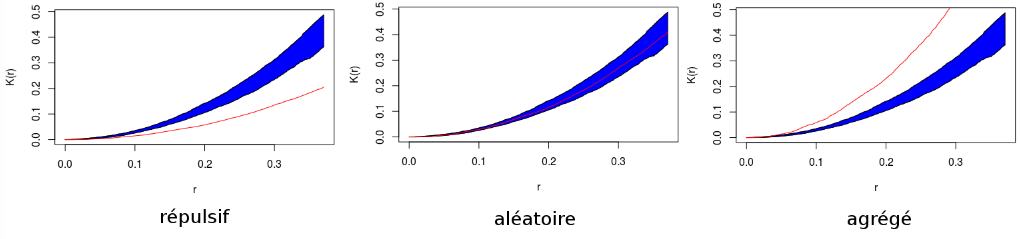
\includegraphics[scale=0.45]{figures/exempleEnveloppes.png}
  \caption{Exemple d'un test d'enveloppe sur la fonction K}
  \label{fig:enveloppeK}
\end{figure}

Ainsi s'il faut analyser une configuration, on peut maintenant comparer sa courbe avec l'enveloppe et faire une analyse plus précise de la répartition. Comme le montre le figure~\ref{fig:enveloppeK}, pour la fonction K: 
\begin{itemize}
\item si la courbe est en dessous de l'enveloppe, la répartition sera plutôt répulsive;
\item si la courbe est dans l'enveloppe, la répartition sera plutôt aléatoire;
\item si la courbe est au dessus de l'enveloppe, la répartition sera plutôt agrégée.\\
\end{itemize}

Remarque: Il n'est pas obligatoire de prendre le minimum et le maximum de chaque fonction pour faire l'enveloppe, on peut très bien faire par exemple un encadrement entre 2.5\% et 97.5\% pour éliminer les valeurs extrêmes.

%%%%%%%%%%%%%%%%

\newpage

%%%%%%%%%%%%%%%%%%%%%%%%%%%%%%%%%%%%%%%%%%%%%%%%%%%%%%%%%%%%%

\chapter{Réalisation}

\section{Environnement logiciel}
Après l'étude mathématique du problème, il fut possible de se consacrer à l'implémentation. Le code du calcul a été écrit en C++ afin d'utiliser un langage compilé connu et utilisé par mon maître de stage et ainsi faciliter l'insertion de mon code dans ses programmes réalisés ultérieurement. La partie graphique (affichage des courbes résultats) a été réalisée avec le logiciel R qui est très utilisé des statisticiens et qui possède une \gls{spatstat}* dédiée aux \gls{PP}s*. Ainsi j'ai pu comparer mes résultats avec ceux de cette librairie.\\

\section{Méthode de travail}

Tout au long du stage nous avons procédé étape par étape. En premier lieu, M. Radu Stoica me donnait des explications, puis me donnait de la documentation à lire sur la partie mathématique dans le livre "Spatial Point Patterns - Methodology and Applications with R"~\cite{BaddEtal16}. 

Ensuite après avoir lu et réfléchi sur une méthode de conception, je la partageais avec lui et nous en discutions. Il me proposait lui aussi des idées et nous regardions si elles pouvaient être inclues dans ma conception. De plus nous réfléchissions également pour savoir si nos méthodes étaient viables et rentables en terme de mémoire ou de temps d'exécution. Ensuite je réalisais le code.

Une fois terminé, ou bien lorsque le travail était suffisamment avancé, je retournais voir M. Stoica pour faire le point. Nous regardions alors ce qui n'allait pas et ce qui pouvait être amélioré. Enfin je corrigeais les défauts de mon code et nous passions à une autre fonction en commençant par la partie théorique.

Ainsi j'ai eu à implémenter les fonctions F, G, J et K expliquées dans la partie 3 du rapport. Ensuite j'ai dû prendre en main du code déjà écrit par M. Stoica afin d'y insérer mes fonctions. Enfin j'ai codé le calcul d'intensité.

%%%%%%%%%%%%%%%%
\section{Structure du code}

Pour réaliser les fonctions j'avais à ma disposition des fichiers texte contenant les valeurs des positions (x,y) d'une répartition de point. J'ai créé un fichier contenant des informations sur des paramètres expérimentaux que l'on pouvait donc modifier d'une expérience à l'autre. Ainsi j'avais 2 fichiers fournisseurs d'informations en entrée.
En analysant les calculs des fonctions, je me suis rendu compte que j'avais besoin de générer plusieurs informations:
\begin{itemize}
\item la surface de la répartition;
\item un quadrillage sur toute la surface pour F;
\item les distances entre chaque point pour K et G;
\item les distances de chaque maille du quadrillage avec chaque point;
\item une liste d'abscisses de rayons.\\
\end{itemize}
Ainsi pour gérer le stockage de ces informations j'ai créé plusieurs \gls{classe}s*. Une fois toutes les \gls{classe}s* instanciées (cf \gls{instance}*) il a fallu les stocker, puis traiter leur valeurs afin d'avoir le matériel nécessaire pour réaliser les calculs. Dans un souci de présentation, je commencerai par présenter les \gls{objet}s* nécessaires aux calculs, puis les algorithmes des calculs, et enfin je parlerai de points plus précis du code. 

\subsection{Création des abscisses}

Pour les calculs des valeurs des fonctions, nous allons faire augmenter un rayon autour de chaque point ou maille. Ce seront les abscisses de nos fonctions. On appelle le dernier rayon, le rayon maximum: "rMAx".

Pour se rapprocher au maximum des courbes fournies par la \gls{spatstat}*, je suis allé chercher des informations sur la façon dont le code crée la liste des rayons (ses abscisses). J'ai alors trouvé sur le site de \gls{spatstat}*\cite{FAQspatstat} qu'il fallait créer une liste de taille 513 (512 intervalles), les valeurs allant de 0 à Rmax.

Le calcul de Rmax est différent pour K et les autres fonctions. Ainsi j'ai trouvé qu'il fallait prendre le quart du plus petit des cotés du rectangle de surface comme rayon maximal pour la fonction K. Cependant, je n'ai rien trouvé pour les autres fonctions.
J'ai donc fait une analyse de la situation: on a vu dans la partie 3 que pour une configuration aléatoire, les fonctions F et G sont définies par l'équation:
\begin{align*}
F_{poiss} = 1-exp(-\lambda.pi.r^2)
\end{align*}
Cette fonction tend vers 1, donc après une certaine abscisse, les valeurs de la fonction seront toutes très proches de 1 et n'ajouteront plus d'information.
On cherche donc un rMax qui permettrait de ne garder que les valeurs inférieures à un gros pourcentage de la valeur finale de la fonction ( > à 90\%)
Alors en notant "P" le pourcentage de la valeur finale on peut écrire:
\begin{align*}
P = 1-exp(-\lambda.\pi.rMax^2)
\end{align*}
Une transformation rapide de l'équation permet d'exprimer clairement rMax en fonction de P:
\begin{align*}
rMax^2 = \frac{-ln(1-P)}{\pi.\lambda}
\end{align*}
Or en choisissant \begin{math}-ln(1-P)=\pi\end{math}:
\begin{align*}
P &= 1-exp(-pi)\\
&=0.9567
\end{align*}
Ainsi avec cette valeur de P on peut avoir un pourcentage de 96\% de la valeur finale tout en ayant un calcul simple de rMax:
\begin{align*}
rMax^2 = \frac{1}{\lambda}
\end{align*}
On a vu également Partie 3, que l'on peut calculer l'intensité \begin{math}\lambda\end{math} par le rapport du nombre de points n sur la taille de la surface W.

Ainsi prendre \begin{math} rMax^2 = \frac{W}{n} \end{math} permet de ne pas avoir de valeur infinie mais de garder la majorité des informations importantes. 


\subsection{Les classes}

Comme le montre le diagramme de \gls{classe}* en Annexe~\ref{fig:diagClasse} j'ai créé 4 \gls{classe}s*.

\subsubsection{La classe Rectangle}
Cette \gls{classe}* se veut être la représentation de la surface. Elle est définie par 4 valeurs d'encadrement de type \gls{double}*:
\begin{itemize}
\item xMin défini par la plus petite valeur de x de la liste de points;
\item xMax défini par la plus grande valeur de x de la liste de points;
\item yMin défini par la plus petite valeur de y de la liste de points;
\item yMax défini par la plus grande valeur de y de la liste de points.\\
\end{itemize}

Ainsi cette \gls{classe}* permet de retourner l'aire totale de la surface nécessaire pour le calcul de K avec un simple calcul:
\begin{lstlisting}[language=C++, caption={Méthode donnant l'aire de la surface}, label={lst:aireSurface}]
double Rectangle::getAire() const{
	return((xMax - xMin)*(yMax - yMin));
}
\end{lstlisting}
    
De plus cette \gls{classe}* permet de renvoyer la distance d'une position à la surface afin de gérer les effets de bord, pour des coordonnées (x,y):
\begin{lstlisting}[language=C++, caption={Méthode donnant la distance d'un point à la surface}, label={lst:distanceSurface}]
double Rectangle::distanceSurface(double x, double y) const{
	double d = xMax - x;
	if(d >= (x - xMin)){
		d = x - xMin;
	}
	if(d >= (yMax - y)){
		d = yMax - y;
	}
	if(d >= (y - yMin)){
		d = y - yMin;
	}
	return d;
}
\end{lstlisting}

\subsubsection{La classe Position}
Cette \gls{classe}* ne sera pas instanciée (cf \gls{instance}*), elle servira de \gls{classe}* mère pour les \gls{classe}s* Point et Quadrillage. Elle est définie par 2 coordonnées "x" et "y" de type \gls{double}* et une valeur de distance au bord de la surface "distanceBord" de type \gls{double}* également.\\

Les \gls{methode}s* de cette \gls{classe}* permettent d'accéder aux variables x,y et distanceBord.


\subsubsection{La classe Point}
Cette \gls{classe}* hérite (cf \gls{heritage}*) de la \gls{classe}* Position, elle se veut être la représentation d'un point de la configuration d'entrée. En plus des caractéristiques de sa \gls{classe}* mère, elle possède la liste "listeDistancePoints" des distances la séparant de chacun des autres points de la configuration.

Cette \gls{classe}* permet alors de trier sa liste de distance de la plus petite à la plus grande afin de faciliter les calculs à venir, la \gls{methode}* utilise le tri du \gls{namespace}* std qui sera expliquée plus en détail page 19.
\begin{lstlisting}[language=C++, caption={Méthode triant la liste de distance}, label={lst:triListe}]
void Point::trierListe(){
	std::sort(listeDistancePoints.begin(), listeDistancePoints.end());
}
\end{lstlisting}

La \gls{classe}* permet également de recupérer un élément précis de sa liste de distance. Comme la liste aura été triée au préalable, plus on augmente l'indice en entrée de la \gls{methode}* plus la valeur retournée sera grande :

\begin{lstlisting}[language=C++, caption={Méthode donnant le ième élément de la liste de distances}, label={lst:getDistanceDuPoint}]
double Point::getDistanceDuPoint(int i){
	return listeDistancePoints[i];
}
\end{lstlisting}


\subsubsection{La classe Quadrillage}
Cette \gls{classe}* hérite (cf \gls{heritage}*) de la \gls{classe}* Position, elle se veut être la représentation d'une maille d'un quadrillage de la surface de la configuration de points. Elle sera utile pour le calcul de la fonction F. En plus des caractéristiques de sa \gls{classe}* mère, elle possède une valeur "distanceVide" de type \gls{double}* qui représente la distance la séparant du point de la configuration dont elle est le plus proche.

Cette \gls{classe}* contient ainsi une \gls{methode}* permettant de trouver le point le plus proche et pour pouvoir initialiser sa variable:

\begin{lstlisting}[language=C++, caption={Méthode trouvant le point le plus proche d'une maille du Quadrillage}, label={lst:setDistanceVide}]
void Quadrillage::setDistanceVide(vector<Point> &point){
	
	int i=0;
	int n = (int)(point.size());
	double dX = 0;
	double dY = 0;
	double distance = 0;
	double dmin = 999999;

	for(i=0;i<n;i++){
		// calcul distances au carré
		dX = x - point[i].getX();
		dY = y - point[i].getY();

		distance = dX*dX + dY*dY;

		if(dmin > distance){
			dmin  = distance ;
		}
	}

	distanceVide = dmin;
}
\end{lstlisting}

Cette \gls{classe}* possède également une \gls{methode}* permettant d'accéder à sa valeur "distanceVide".

\subsection{Algorithmes de calcul des fonctions}
Les algorithmes de calcul des fonctions K et F,G,J sont représentés en Annexe~\ref{lst:algoK} et~\ref{lst:algoFGJ}. On suppose qu'on a préalablement rangé et trié les valeurs des distances à comparer.

Pour K, on procède point par point: on calcule combien chaque point a de voisins pour chaque rayon. Si un point est trop près du bord par rapport à la taille d'un rayon, on n'ajoute pas son nombre de voisins. La liste des points étant préalablement triée par rapport à leur distance au bord, on peut arrêter la boucle sur les points dès qu'un point n'est plus dans la zone de sûreté.\\
De même en ayant trié les distances entre les points, on peut arrêter la boucle sur les distances aux autres points dès qu'une distance dépasse la valeur de rayon. On peut alors garder la valeur du nombre de voisins, et reprendre le calcul pour rayon suivant plus grand.
En effet, comme les listes ont étés préalablement triées, une fois la valeur de rayon dépassée toutes les valeurs suivantes le seront aussi.

Pour F,G et J, on procède point par rayon: pour chaque rayon, on calcule la valeur de F et de G puis on en déduit la valeur de J. Ainsi on compare la valeur de chaque rayon avec les valeurs de distance du plus proche voisin de chaque point pour G et de chaque quadrillage pour F. De plus comme pour K, en triant les listes de Point et de Quadrillage en fonction de leur distance au bord, on peut optimiser les calculs de correction d'effet de bord.

\subsection{Les listes}

Présent à plusieurs endroit du code, l'\gls{objet}* Vector du \gls{namespace}* std m'a été très utile. En effet, c'est ce type de liste que j'ai utilisé pour:
\begin{itemize}
\item la liste de Point;
\item la liste de Quadrillage;
\item chaque liste de distance dans les \gls{objet}s* Points;\\
\end{itemize}

Comme on peut le voir sur le site cppreference.com\cite{vector} l'\gls{objet}* Vector est un conteneur séquentiel qui encapsule les tableaux de taille dynamique.

Comme les tableaux, l'\gls{objet}* Vector utilise un stockage contigu, ce qui signifie que les éléments sont accessibles non seulement via les itérateurs, mais aussi à partir des pointeurs classiques sur un élément. A la différence des tableaux, la taille du vecteur peut être modifiée dynamiquement, c'est à dire que son stockage est pris en charge automatiquement, pouvant être augmenté ou diminué au besoin.

Les complexités des opérations courante pout l'\gls{objet}* Vector sont les suivantes :
\begin{itemize}
\item Accès aléatoire - constante O(1);
\item Insertion ou le retrait d'éléments à la fin - constante amortie O(1);
\item Insertion ou le retrait d'éléments - linéaire O(n);\\
\end{itemize}

Au vu du nombre important d'accès aux valeurs des listes pour les calculs, le choix de cette structure m'a paru adapté.

\subsection{Les tris}

Trier les listes définies ci-dessus, permet par la suite d'éviter de nombreux calculs liés aux distances entre les points.

Il a ainsi fallu \gls{classe}r* les listes de Point et de Quadrillage de l'\gls{objet}* le plus éloigné du bords au plus proche pour les deux listes. De plus pour chaque \gls{objet}* Point il a fallu trier la liste de distance aux autres points de la plus petite à la plus grande.

La méthode de tri utilisée fut la \gls{methode}* "sort" du \gls{namespace}* std. Selon le site cppreference.com\cite{sort} c'est un tri optimisé qui utilise l'algorithme de tri "introsort" hybride entre le tri rapide et tri par tas. Il fournit ainsi une vitesse de calcul rapide pour le cas moyen, et des performances optimales dans le pire des cas. Ce tri possède ainsi une complexité de \begin{math}n.log(n)\end{math} dans tous les cas.

L'étude\cite{PerfSort} menée par une élève de l'ISIMA, à Clermont-Ferrand montre les avantages et efficacité de cette méthode de tri sur l'\gls{objet}* Vector du \gls{namespace}* std.


%%%%%%%%%%%%%%%%

\section{Stratégies d'implémentations adaptées au problème}


\subsection{Le remplissage des listes des distances}
Comme chaque point possède la liste des distances aux autres points, on peut se représenter le tableau suivant:\\
\hspace*{3cm}
\begin{tabular}{c|cccccc}
   & point 1 & point 2 & ... & point j & ... & point n \\
  \hline
  point 1 & 0 & \begin{math} d_{12} \end{math} & ... & \begin{math} d_{1j} \end{math} & ... & \begin{math} d_{1n} \end{math} \\
  point 2 & \begin{math} d_{21} \end{math} & 0 & ... & \begin{math} d_{2j} \end{math} & ... & \begin{math} d_{2n} \end{math}\\
  ... & ... & ... &  ...  & ... & ... & ... \\
  point i & 0 & \begin{math} d_{i2} \end{math} & ... & \begin{math} d_{ij} \end{math} & ... & \begin{math} d_{in} \end{math} \\
   ... & ... & ... & ... & ... & ... & ... \\
  point n & \begin{math} d_{n1} \end{math} & \begin{math} d_{n2} \end{math} & ... & \begin{math} d_{nj} \end{math} & ... & 0 \\
\end{tabular}

Or la distance d'un point i à un point j est la même que celle d'un point j à un point i, c'est à dire que \begin{math} d_{ij} = d_{ji}\end{math}. On n'a besoin de ne calculer que la partie triangulaire supérieure du tableau pour avoir toutes les valeurs.\\

\begin{lstlisting}[language=C++, caption={Remplissage des listes de distance}, label={lst:distances}]
int i;
int j;
double dX = 0;
double dY = 0;
double distance = 0;

for( i = 1; i < n-1; i++){
    for( j = i; j < n; j++){
        dX = point[j].getX() - point[i].getX();
		dY = point[j].getY() - point[i].getY();

 		distance  = dX*dX + dY*dY ;
 		
 		point[i].ajoutDistance( distance );
        point[j].ajoutDistance( distance );
    }
}
\end{lstlisting}

Ainsi en appliquant la méthode ci dessus, on peut faire moitié moins d'opérations: pour n points, on économise n(n-1)/2 opérations.

\subsection{Les distances aux carrés}

La majorité des calculs concerne des calculs de distance. Ainsi entre 2 points A et B d'abscisses et d'ordonnées respectives (xA,yA) et (xB,yB) la distance se calcule par la formule de Pythagore:
\begin{align*}
distance = \sqrt{(xB-xA)^2 + (yB-yA)^2}
\end{align*}
Or le calcul de la racine carrée prend du temps et peut être évité.\\

En effet, ces distances vont être par la suite seulement comparées, ainsi pour un rayon "r" et une distance entre 2 points "d":
\begin{align*}
d < r  \Leftrightarrow  d^2 < r^2
\end{align*}
Ainsi, il est utile de ne stocker que les valeurs au carré des calculs de distance. En notant ts le temps de calcul d'une racine carrée, on gagne les temps t :

\hspace*{1cm} t = (n*(n-1)/2)*ts \hspace*{1cm} pour les calculs de distance point/point

\hspace*{1cm} t = (m*n)*ts \hspace*{1cm} pour les calculs de distance maille/point\\

\subsection{Arrêter les calculs et stockage au rayon maximal}
Pour le calcul de K, pour chaque point on incrémente un compteur selon le nombre de voisins qu'a le point étudié dans un certain rayon. Tous les points à une distance plus grande que le plus grand rayon rMax ne seront donc jamais pris en compte. Ainsi lors du remplissage des listes de distance, il est inutile de stocker les distances entre 2 points éloignés de plus de rMax. Cela permet d'économiser beaucoup de mémoire, mais aussi de réduire drastiquement le temps de calcul:  moins de temps d'ajout dans les listes, des tris plus rapides et moins de calculs à la fin.

\section{Tests d'enveloppe}

Monsieur Stoica avait par le passé réalisé des programmes en C++ permettant de générer des configurations de points que l'on sait être plutôt répulsifs ou plutôt agrégés. Ses programmes au nombre de deux suivent les méthodes de "Strauss" et de "Area Interaction". Ainsi "Strauss" génère à chaque lancement des configurations de points répulsives, tandis que "Area Interaction" génère
des configurations répulsives ou agrégées selon les paramètres fournis.

En itérant un certain nombre de fois ces programmes, on peut alors faire des enveloppes en appliquant à chaque itération les programmes des fonctions F, G, J et K. On change alors la référence Poissonnienne (qui modélise un phénomène aléatoire), on utilise une référence du phénomène de répulsion et une référence du phénomène d'agrégation.

J'ai alors dû explorer le code de M. Stoica, afin d'y insérer et d'y adapter mes programmes. Ainsi en bouclant l'exécution du code obtenu, on peut stocker les valeurs nécessaires pour afficher les enveloppes.

\section{Intensité}

%Le calcul de l'intensité d'une réalisation de processus ponctuel est un calcul séparé des fonctions implémentées précédemment.

\subsection{Calcul}

Pour le calcul de l'intensité j'ai gardé la \gls{classe}* Point pour modéliser les points de la réalisation et la \gls{classe}* Rectangle pour modéliser la surface.
Ainsi après une lecture des paramètres, tous les \gls{objet}s* nécessaires à l'implémentation sont disponibles. L'algorithme se trouve en Annexe~\ref{lst:calculIntensite}.
    
Le principe est donc de se placer sur toutes les positions de matrice quadrillée et de calculer les valeurs des intensités en chacune de ces positions. Les valeurs des intensités sont mesurées en fonction du nombre de points à proximité des positions. Ainsi en utilisant les fonctions noyaux décrites au 3.2 on compare la position avec celle de tous les points de la réalisation. L'implémentation de ces fonctions est représentée ci-dessous:

\begin{lstlisting}[language=C++, caption={Fonctions des noyaux carré, rond et Gaussien}, label={lst:fonctionsNoyaux}]
double indicatriceCarre(double u1, double u2, double c){
	return ( (u1 < c) && (-u1 < c) && (u2 < c) && (-u2 < c) ) ? 1 : 0;
}

double indicatriceRond(double u1, double u2, double r){
	return ( (u1*u1 + u2*u2)/4 <= r*r ) ? 1 : 0;
}

double gaussienne(double u1, double u2, double sigma){
	return exp(-(u1*u1 + u2*u2)/(2*sigma*sigma));
}
\end{lstlisting}


\subsection{Correction des bords}

Ensuite comme expliqué au 3.2, les estimations sont faussées par des effets de bords. La correction à appliquer est une division que l'on voit apparaître dans l'algorithme en Annexe~\ref{lst:calculIntensite}, et qui est noté "Erreur()". Cette erreur ne dépend que de la position d'un point. Ainsi en début de programme il a fallu calculer ces erreurs.

La formule mathématique pour ce calcul est utilise la fonction noyau. Comme le noyau Gaussien est le plus intéressant des trois, la correction n'a été appliquée que sur ce noyau. Ensuite il y a un calcul d'intégrale (continue), il faut donc utiliser une méthode de discrétisation pour calculer numériquement cette intégrale. Selon le tableau comparatif de cette page Wikipédia\cite{Integrales}, la méthode de Rohmberg converge le plus rapidement vers une solution précise.

Cette méthode génère un tableau triangulaire d'estimations numériques de l'intégrale en appliquant l'\gls{richardson}* à la \gls{trapeze}*. Cela permet d'améliorer l'ordre de convergence de la \gls{trapeze}* en divisant l'intervalle d'étude et en formant des combinaisons judicieuses des différents termes calculés \cite{Rohmberg}.

Le principe est le suivant : si l'on veut trouver une estimation de $f(x)$ intégrée de $a$ à $b$ on calcule le premier terme $R(0,0)$ par la méthode des trapèzes, puis les termes suivants en sommant des nouveaux termes et en faisant des combinaisons avec les termes calculés précédemment : 
\begin{align*}
R(0,0) &= \frac{1}{2}(b - a)(f(a) + f(b))\\
R(n,0) &= \frac{1}{2}R(n-1,0) + h \sum_{k=1}^{2^{n-1}}f(a + (2k - 1)h)\\
R(n,m) &= \frac{1}{4^m-1}(4^m R(n,m-1) - R(n-1,m-1))\\
\end{align*}
avec \begin{math}h = (b-a)/2^n, n \geq 1, m \geq 1\end{math}.

On utilise alors les termes diagonaux $R(n,n)$ comme estimation de l'intégrale avec une erreur en $O(h^{2n+1})$.

L'intégrale étant sur une surface (intégrale double), il a fallu faire deux fonctions pour la méthode de Rohmberg. Une première fonction fait varier une première variable et appelle une deuxième fonction qui, elle, fait varier une deuxième variable et appelle la fonction du noyau.

%%%%%%%%%%%%%%%%%%%%%%%%%%%%%%%%%%%%%%%%%%%%%%%%%%%%%%%%%%%%%

\chapter{Bilan}

\section{Résultats obtenus}

\subsection{Validation}

Une fois les fonctions réalisées, il a fallu s'assurer de la qualité des résultats. Pour cela je me suis aidé de la \gls{spatstat}* pour comparer les courbes obtenues avec mes calculs avec celles réalisées par leurs algorithmes.

Comme on peut le voir en Annexe~\ref{fig:compSpatstat} le résultat final correspond bien aux attentes. Il est difficile de distinguer à l'oeil les écarts entre les courbes, sauf pour la fonction J pour laquelle la différence est engendrée par les petits écarts sur les fonctions F et G. On a alors étudié les écarts entre les valeurs calculées par mon programme et celles calculées par \gls{spatstat}*. Le tableau~\ref{tab:stats} ci-dessous recense, pour ces écarts de résultats, les moyennes, maximums et écarts types pour chaque fonction.

\begin{table}[ht]
    \centering
    \begin{tabular}{|c|c|c|c|}
          \hline
          fonction & moyenne & valeur maximale & écart type \\
          \hline
          $f_{ecart}$ & 0.001407488 & 0.005637747 & 0.001034606 \\
          \hline
          $g_{ecart}$ & 1.500446e-05 & 0.0003938599 & 5.073528e-05 \\
          \hline
          $j_{ecart}$ & 0.0004730104 & 0.004047371 & 0.0007574491 \\
          \hline
          $k_{ecart}$ & 0.002176537 & 0.006467136 & 0.001847468\\
          \hline
    \end{tabular}
    \caption{Statistiques sur les écarts de résultats}
    \label{tab:stats}
\end{table}
Ainsi les écarts moyens de résultats ne dépassent pas un ordre de grandeur de $10^{-3}$, écarts considérés satisfaisant par M. Stoica. De plus les valeurs maximales de ces écarts indiquent que dans le pire des cas les écarts sont raisonnables. Les écarts types montrent que les valeurs ne s'éloignent pas beaucoup de la moyenne. On peut donc considérer les calculs de fonction comme valides.

%%%%%%%%%%%%%%%%%%%%%%%%%

\subsection{Visualisation}

Les codes en C++ écrivent des valeurs dans un fichier texte, ces valeurs sont ensuite lues par un programme R qui traite alors les résultats. Ensuite, une fois les résultats rapidement analysés (recherche des minimums et maximums pour le test d'enveloppe), ce même programme affiche les courbes résultantes des valeurs calculées par le premier programme.

En Annexe~\ref{fig:compPoisson} sont représentés les résultats des calculs des fonctions F,G,J et K avec leur courbes des valeurs pour un aléatoire théorique pour une observation. Ainsi on peut constater que cette distribution est un peu plus répulsive que ne le serait une distribution complètement aléatoire.

En Annexe~\ref{fig:testEnveloppe} est représenté le résultat des tests d'enveloppe. La dernière courbe analysée y est représentée également en tant qu'exemple.

En Annexe~\ref{fig:testIntensite} est représenté le résultat d'un calcul d'intensité avec un noyau carré, rond et Gaussien. La correction des bords n'est montrée que pour le noyau Gaussien car c'est le plus intéressant.

%%%%%%%%%%%%%%%%%%%%%%%%%

\subsection{Utilisation}

Vous pouvez trouver le projet en libre accès sur github, à l'adresse:\\
\hspace*{2cm} \url{https://github.com/DugueC/Stage2A}\\

Les codes fonctionnent à condition d'avoir installé un compilateur c++ et R.\\
Si un script ne fonctionne pas, essayez de donner les droits au fichier\\ ( chmod 777 nom\_script.sh ).

Les procédures d'utilisations des programmes sont décrites dans le "READ ME".

%%%%%%%%%%%%%%%%%%%%%%%%%

\section{Difficultés et Solutions}

Les premières difficultés sont intervenues dès le début du stage. N'étant pas à l'aise avec le langage C++, et ne connaissant pas le langage R, j'ai dû m'adapter et me documenter. J'ai également demandé de l'aide au début pour l'affichage des fonctions réalisé en R. La barrière du langage à donc freiné dans un premier temps l'avancée du projet.

Une fois les fonctions réalisées en procédant simplement par un suivi intuitif des équations des fonctions théoriques, il a fallu accélérer les temps de calculs. En effet mon programme n'était pas très performant dès que les configurations de points étaient trop fournies, car il n'était pas optimisé dans une optique de gain de temps. J'ai donc revu mes algorithmes et trouvé des astuces afin que le temps de calcul des fonctions soit du même ordre que ceux réalisés par la \gls{spatstat}*. Cela n'a pas toujours été facile notamment pour les changements d'algorithmes.

%%%%%%%%%%%%%%%%%%%%%%%%%

\section{Devenir du projet}

L'ensemble du projet a été réalisé en 2 dimensions, c'est à dire que les points fournis n'avaient que deux coordonnées spatiales. Une adaptation du code pour une 3ème dimension ouvrirait la porte à un nouveau panel d'expériences qu'il serait possible d'analyser.

M. Radu Stoica s'intéresse à la répartition des positions des galaxies dans notre univers. Au fur et à mesure que les nouveaux outils mathématiques sont proposés, cela demande leur reformatisation. Une perspective immédiate est d'étendre ces développements logiciels au cas des \gls{PP}s* in\gls{homogene}s*.

%%%%%%%%%%%%%%%%%%%%%%%%%%%%%%%%%%%%%%%%%%%%%%%%%%%%%%%%%%%%%

\chapter{Conclusion}


L'objectif de ce stage à été atteint: les outils informatiques pour traiter les données ponctuelles ont été réalisés (fonctions F,G,J et K) et intégrés au code de mon maître de stage afin d'analyser ces données (test d'eveloppe). Il a été possible également d'implémenter des calculs d'intensité durant ce stage de 8 semaines.

Pour le futur, on peut envisager une extension des fonctions implémentées pour des données en trois dimensions. De même on pourrait continuer ce projet en élargissant son développement pour des processus in\gls{homogene}s*.
 
Finalement cette expérience m'a fait découvrir un monde de la recherche en mathématique et un nouveau mode de travail. Ce fut donc une expérience agréable et utile pour moi puisqu'il m'a permis d'apprendre le langage R et de m'améliorer dans le C++ et d'envisager un nouvel axe de projet professionnel.

\cleardoublepage

%%%%%%%%%%%%%%%%%%%%%%%%%%%%%%%%%%%%%%%%%%%%%%%%%%%%%%%%%%%%%


\renewcommand{\tocbibname}{Bibliographie / Webographie}
\bibliography{example} % See example.bib 
\bibliographystyle{plain}

\cleardoublepage

%%% liste des illustrations
\listoffigures
\cleardoublepage

%%% liste de tableaux
\listoftables
\cleardoublepage

%%% liste des algos et codes
\lstlistoflistings
\cleardoublepage

%%% Glossaire
%\chapter*{Glossaire}
\printglossaries
\addcontentsline{toc}{chapter}{Glossaire}
\cleardoublepage


\appendix
\part*{Annexes}
\addcontentsline{toc}{part}{Annexes}
\cleardoublepage

\chapter{Diagramme de Classes}
\begin{figure}[h]
 \centering
  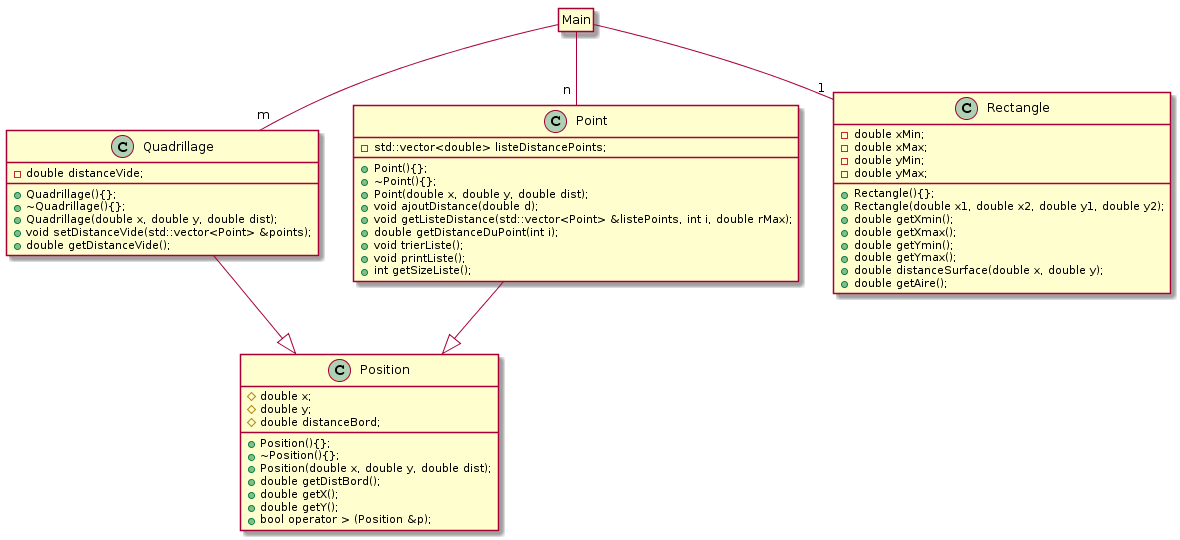
\includegraphics[scale=0.43]{figures/diagrammeClasses.png}
  \caption{Diagramme de classe pour les calculs des fonctions}
  \label{fig:diagClasse}
\end{figure}
\cleardoublepage


\chapter{Algorithmes des calculs des fonctions}
\lstset{
    keywordstyle=\bfseries,
    morekeywords={ ENTREE, CONSTANTES, LISTES, POUR, TANT, QUE, INCREMENTER, ET, SAUVEGARDER, VARIABLES, SI, SINON},
}

\begin{lstlisting}[ caption={Algorithme fonction K}, label={lst:algoK}]
ENTREE : Liste des Points

CONSTANTES :
    n = nombre de points dans liste
    nR = nombre de rayons à analyser
    aire = aire de la surface couverte par les points de la liste

LISTES : 
    NombrePointsConsideres[]
    Kcumule[]
    
VARIABLES :
    i = 0
    j = 0
    k = 0

POUR ( i de 0 à n )
{
    j = 0
    
    TANT QUE ( distance du point i au bord  >  au j-eme rayon )
          ET ( j < nR )
    {
        INCREMENTER NombrePointsConsideres[j]
         
        TANT QUE ( distance du point i au point k < j-eme rayon)
              ET ( k < n - 1 )
        {
            INCREMENTER k
        }
        
        Kcumule[j] = Kcumule[j] + k
        
        INCREMENTER j
    } 
}
    
POUR ( j de O à nR )
{
		SAUVEGARDER K[j] = Kcumule[j]*aire/((n-1)*NombrePointsConsideres[j])
}

\end{lstlisting}

\cleardoublepage

\begin{lstlisting}[ caption={Algorithme fonction F, G et J}, label={lst:algoFGJ}]
ENTREE : Liste des Points

CONSTANTES :
    nP = nombre de points dans liste
    nQ = nombre de quadrillage
    nR = nombre de rayons à analyser
    aire = aire de la surface couverte par les points de la liste

VARIABLES :
    i = 0
    j = 0
    k = 0
    sommeF = 0
    sommeG = 0

POUR ( k de 0 à nR )
{
    i = 0
    
    TANT QUE ( distance du point i au bord  >=  au k-eme rayon )
          ET ( i < nP )
    {
        SI ( distance du point i au plus proche point voisin <= k-eme rayon)
        {
            INCREMENTER sommeG
        }
        INCREMENTER i
    }
    
    j = 0
    
    TANT QUE ( distance du quadrillage j au bord  >  au k-eme rayon )
          ET ( j < nQ )
    {
        SI ( distance du quadrillage j au plus proche point voisin <= k-eme rayon)
        {
            INCREMENTER sommeF
        }
        INCREMENTER j
    }
    
    SAUVEGARDER G = sommeG/i
    SAUVEGARDER F = sommeF/j
    
    SI ( F==1 )
    {
        SAUVEGARDER J = INFINI
    }
    SINON
    {
        SAUVEGARDER G = (1-G)/(1-F)
    }
}
\end{lstlisting}

\cleardoublepage
~
\vspace{3cm}
\begin{lstlisting}[ caption={Algorithme calcul de l'intensité}, label={lst:calculIntensite}]
ENTREE : Liste des Points, Liste des Erreurs, fonction Noyau()

CONSTANTES :
    m = nombre pour avoir une matrice de quadrillage de taille m x m
    n = nombre de points
    aire = aire de la surface couverte par le noyau
    sigma = constante pour la fonction Noyau

VARIABLES :
    i = 0
    j = 0
    k = 0
    x = 0
    y = 0
    intensite = 0


POUR ( i de 0 à m )
{

	POUR ( j de 0 à m )
	{
        intensite = 0;
        
        // pour tous les points
        POUR ( k de 0 à n )
        {
            // calcul de l'ecart entre la position du quadrillage (i,j)
            // et la position du point k stocke dans les variables x et y
            (x,y) = CALCUL_ECART(i,j,k)
            
            intensite = intensite + Noyau(x,y,sigma)/Erreur(k)
        }
        
        // écriture des calculs
        SAUVEGARDER intensite/aire
	}
}
\end{lstlisting}

\cleardoublepage

\chapter{Représentations sous R}

\begin{center}
\begin{figure}[h]
  \centering
  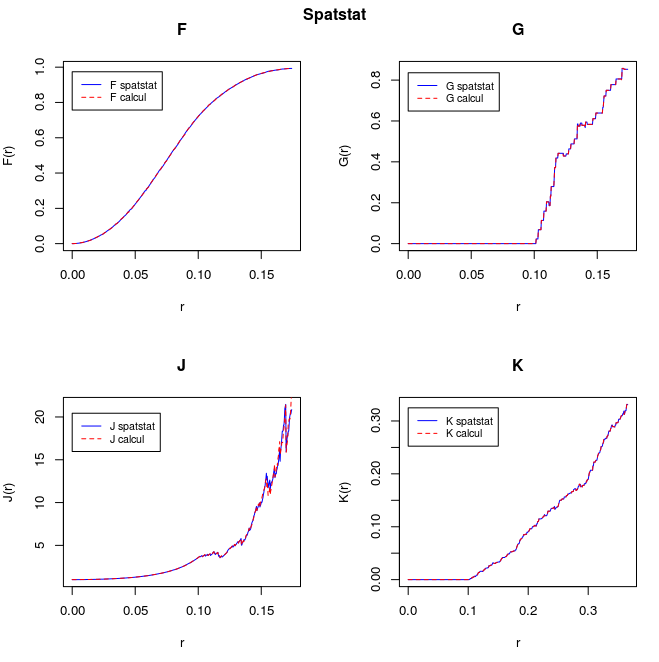
\includegraphics[scale=0.7]{figures/calcul&spatstat.png}
  \caption{Comparaison des fonctions programmées avec celles calculées par spatstat }
  \label{fig:compSpatstat}
\end{figure}
\end{center}

\cleardoublepage

\vspace*{2cm}
\begin{center}
\begin{figure}[h]
  \centering
  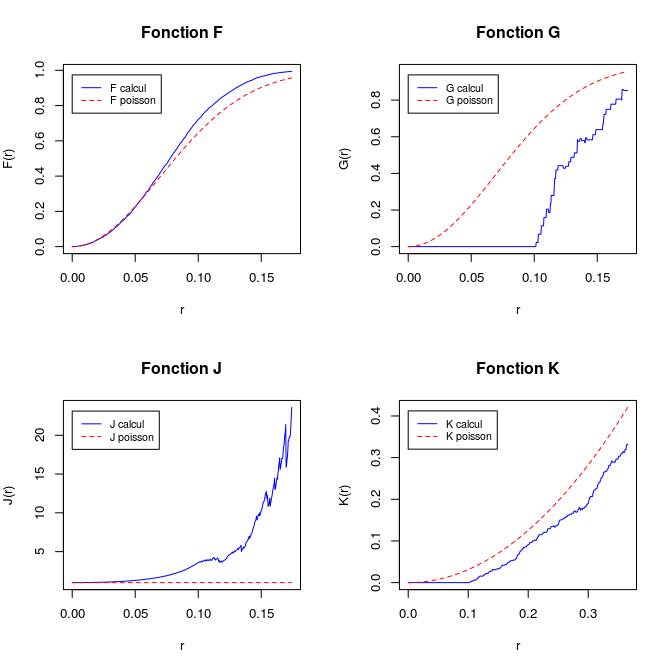
\includegraphics[scale=0.7]{figures/calcul&poisson.png}
  \caption{Comparaison des fonctions programmées avec courbes théoriques pour une répartition aléatoire}
  \label{fig:compPoisson}
\end{figure}
\end{center}

\cleardoublepage

\vspace*{2cm}
\begin{center}
\begin{figure}[h]
  \centering
  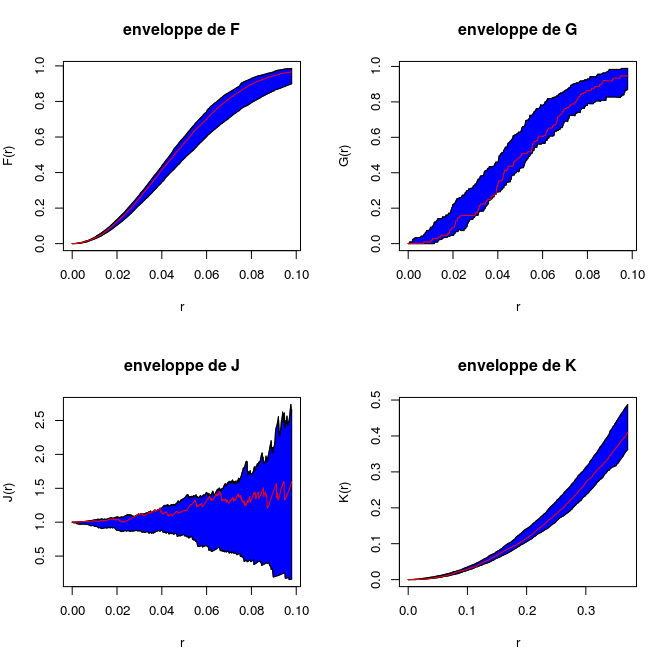
\includegraphics[scale=0.7]{figures/calculEnveloppes.png}
  \caption{Exemple de résultat des tests d'enveloppes}
  \label{fig:testEnveloppe}
\end{figure}
\end{center}

\cleardoublepage

\vspace*{2cm}
\begin{center}
\begin{figure}[h]
  \centering
  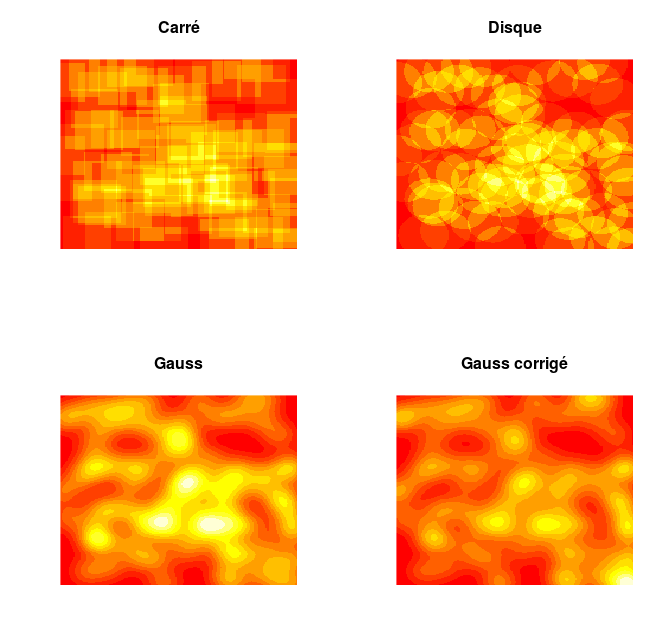
\includegraphics[scale=0.7]{figures/intensite.png}
  \caption{Exemple de résultat des calculs d'intensité}
  \label{fig:testIntensite}
\end{figure}
\end{center}

\cleardoublepage

\thispagestyle{empty}

\section*{Résumé}
\addcontentsline{toc}{chapter}{Résumé}

Ce rapport présente le travail de stagiaire effectué dans l'équipe Probabilité-Statistique de l'Institut Elie Cartan de Lorraine. Ce projet s'inscrit dans le cadre d'un stage de 2ème année à TELECOM Nancy. Le stage a pour but la création d'outils informatiques pour traiter et analyser des données spatialisées en utilisant des \gls{PP}s*. Les fonctions à implémenter testent si les points d'une configuration sont plus ou moins répartis aléatoirement.\\

Avec une génération de répartitions ponctuels créé par M. Radu Stoica, il est possible de faire une enveloppe de valeurs qui permet d'avoir une estimation plus précise de la tendance de répartition des points. Ainsi, les résultats de ce projet permettrons à M. Stoica de faire de futures analyses de situations plus précises.\\

{\bf Mots-clés : statistique, analyse, processus ponctuel }


\section*{Abstract}
\addcontentsline{toc}{chapter}{Abstract}

This report present a trainee work for the Probability-Statistique team of the "Institut Elie Cartan de Lorraine". This project was realised in the framework of a 2nd year trainee in TELECOM Nancy. The goal of the traineeship is to create a computer tool in order to treat and analyze spatial data using point process. The functions to develop intend to estimate the ramdom degree of a point pattern.

With a point pattern generator created by Mr Radu Stoica, it is possible to make a data envelop which allow a more precise estimation of the point repartition trend. Thus, the results of this project would allow Mr Stoica to carry out  more precise analysis in the futur.

{\bf Keywords : statistic, analysis, point process}

\end{document}